%!TEX root=./pfc.tex
\chapter[Implementación del sistema]{\label{}
Implementación del sistema}

La vista de implementación se ocupa de la gestión de la configuración de las partes del sistema (componentes), las cuales pueden ensamblarse de diferentes formas para obtener el sistema ejecutable.

De esta manera, los diagramas de componentes aparecen cuando se modelan los aspectos físicos de los sistemas orientados a objetos. Así, los diagramas de componentes muestran la organización y las dependencias entre un conjunto de componentes y se utilizan para modelar la vista de implementación estática de un sistema.

Por tanto, ahora se va a comentar el diagrama de componentes asociado al sistema para especificar la implementación del sistema.

\begin{figure}[h]
	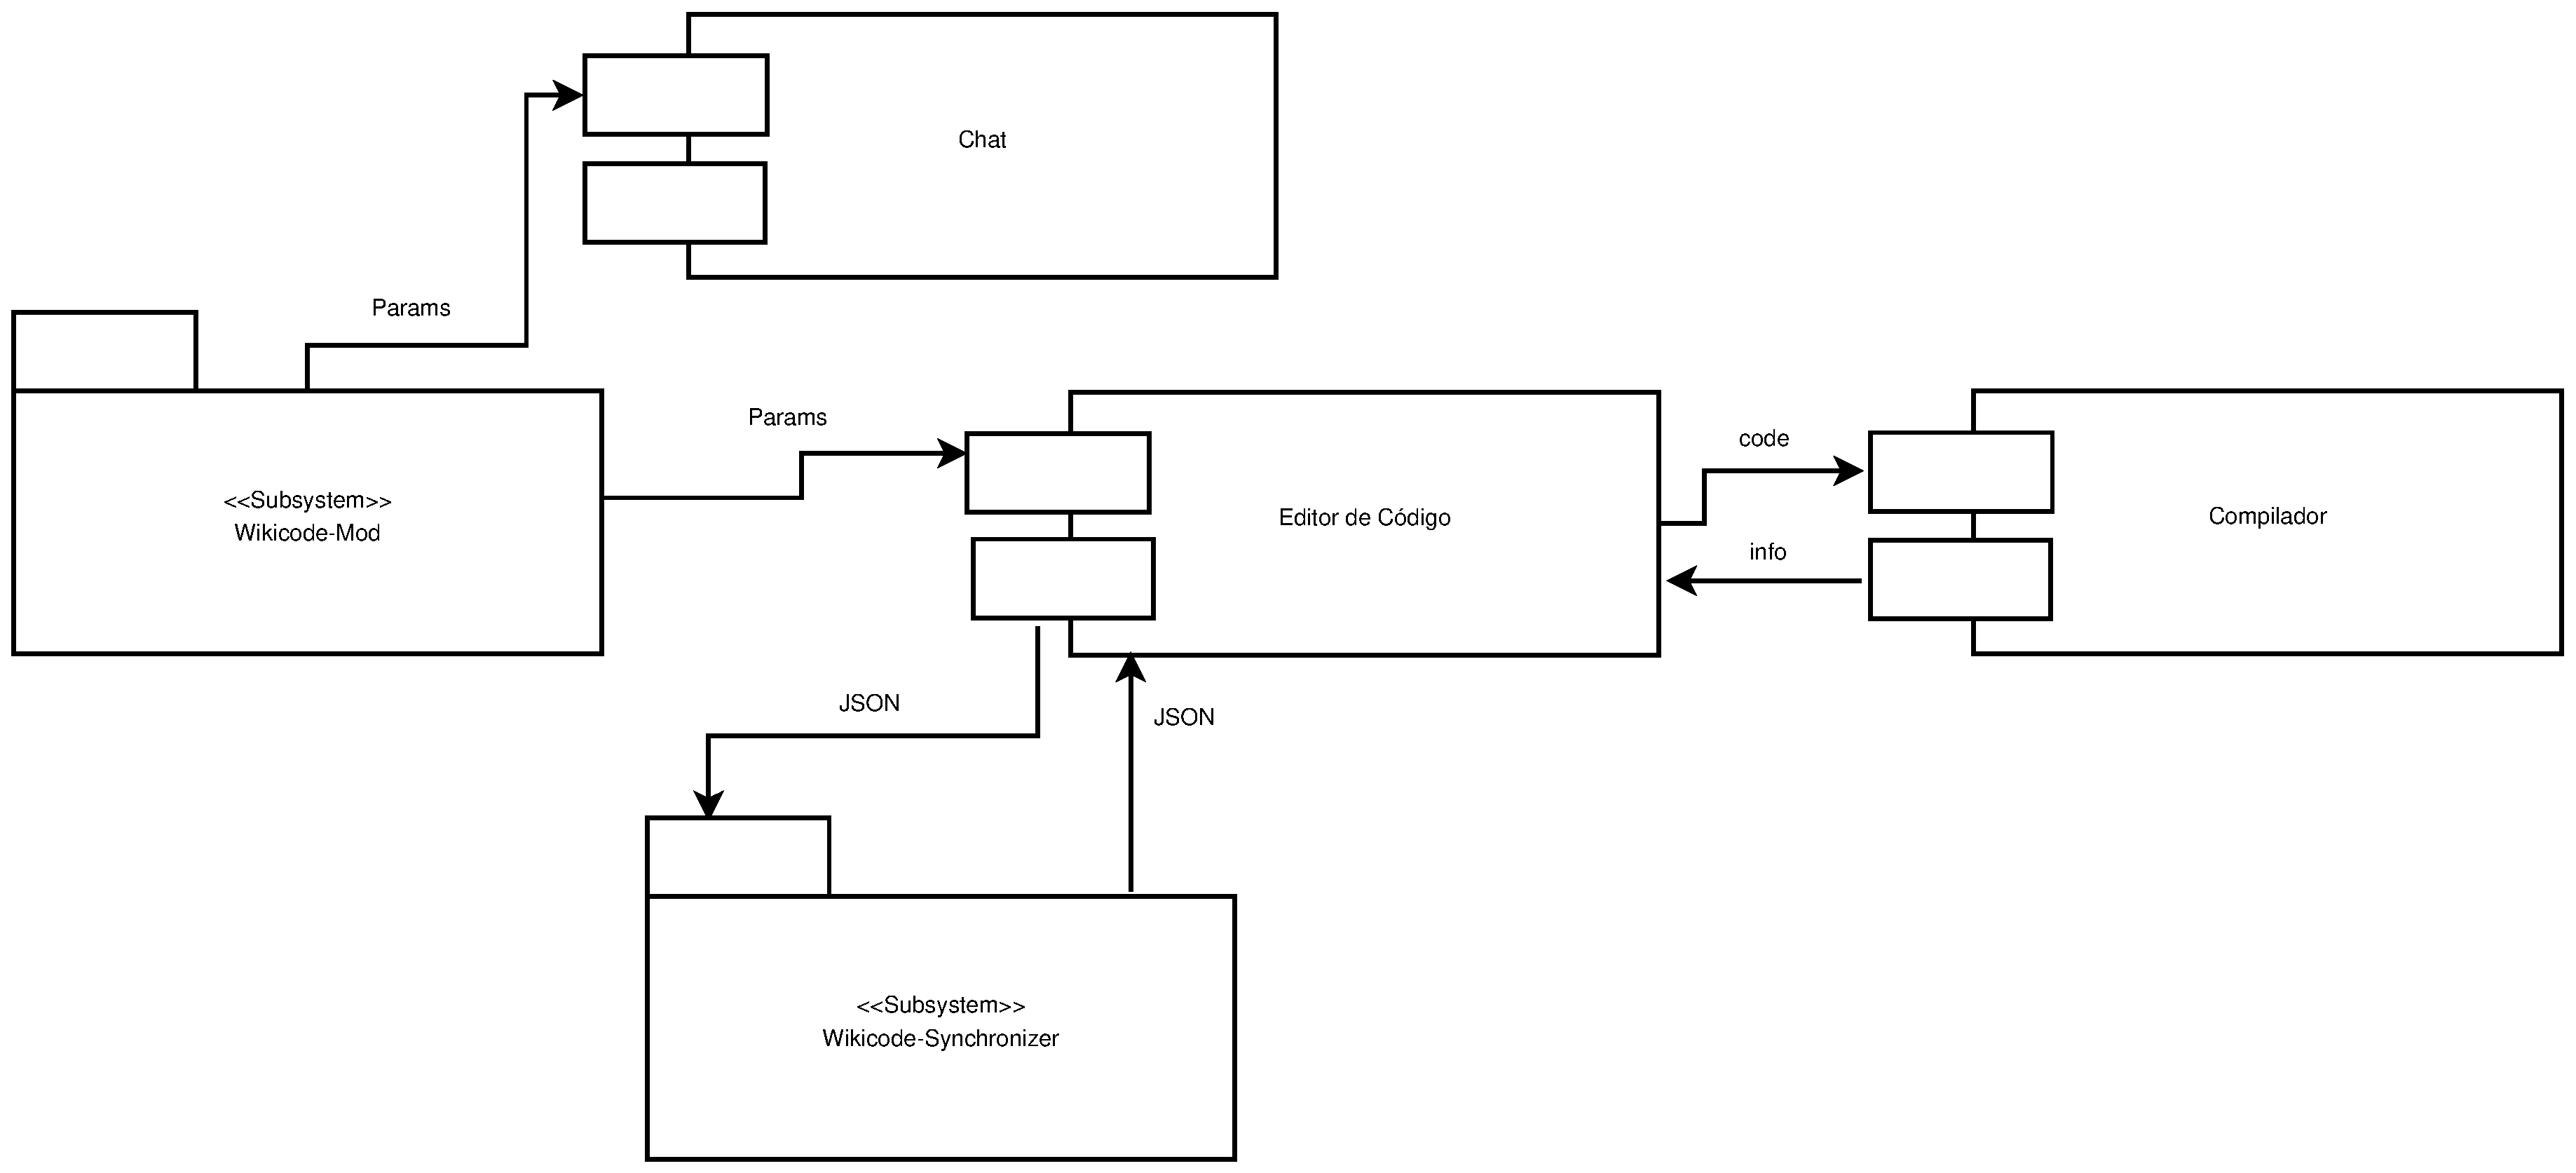
\includegraphics[width=\textwidth]{./img/componentes.eps}
	\caption{Diagrama de Componentes}
\end{figure}